\documentclass[a4paper, 11pt]{article}
\usepackage{comment} % enables the use of multi-line comments (\ifx \fi) 
\usepackage{lipsum} %This package just generates Lorem Ipsum filler text. 
\usepackage{fullpage} % changes the margin
\usepackage{graphicx}
\usepackage{cellspace}
\setlength\cellspacetoplimit{4pt}
\setlength\cellspacebottomlimit{4pt}

\usepackage{titlesec}
\setcounter{secnumdepth}{4}

\newcommand\cincludegraphics[2][]{\raisebox{-0.3\height}{\includegraphics[#1]{#2}}}

\usepackage[english]{babel}
 
\usepackage{minted}

\setlength{\parindent}{4em}
\setlength{\parskip}{1em}
\renewcommand{\baselinestretch}{1.25}

\begin{document}
%Header-Make sure you update this information!!!!
\noindent
\large\textbf{Data Visualisation Report} \hfill \textbf{Antonio Gargaro} \\
\normalsize F21DV \\
Prof. Mike Chantler  \hfill Due Date: 19/11/18  \\

\tableofcontents
\newpage

\section{Executive Summary}
% MAX 1 PAGE
% This section concisely describes goals for the project and major findings and lessons learnt
The development of a dashboard to display concise topic model data intuitively to represent rankings against word count for `Unit of Assessments', geographical focus of these units, and the weighting of the top three word collections per unit. Originally, the data provided was separate and would require users a lot of time to research and gather each document. Analysis of each document is another encumbering task in of itself. Displaying relations clearly between this data is the aim of this project.

Utilising `d3.js' and the examples provided by Mike Chantler, Mike Bostock and other `blo.cks.org' authors allows for a clear resolution towards representing this data. Specifically, licensed code was modified within the bounds of the specified license, where each source file has descriptor headings for this. Most source files are based off of Mike Chantler's work. The need to quickly filter through nested data of institutions requires the power of d3 and JavaScript to carry out data manipulation and graph these data points meaningfully in a web browser.

I find that this is possible by following the `General Update Pattern' described by Chantler and Bostock. This allows for the reuse and addition of data with efficiency to ensure an optimal experience. There is many methods provided by the d3 library to display this data in intuitive and clear ways. I ultimately decided on a sunburst for navigation, a scatter plot for comparisons and a force-directed graph for relations and comparisons.

Ultimately, d3 provides a large set of tools to complete this project. This is apparent with the ability to modify all aspects of chart generation, the ability to select specific elements already displayed and modify them, as well as the possibility of moving objects across the screen to provide an interactive experience.

\newpage
\section{Interface Design: Rationale \& Critical Review}

A large sunburst displaying all institutions allows for quick access to any specific one. A `breadcrumb' trail allows the user to keep track of where they are in this hierarchy, a legend gives a quick reference about which region matches to what colour, and an interactive map displaying what town is represented by each slice. This displays a clear navigational hierarchy for the DoR user to select specific regions, towns or institutions, while understanding what area of the UK he is searching in. 

A scatter plot graph represents all the unit of assessment documents from one of the selected institutions. The `4* Rating' is plotted against the word count for each document. This allows the DoR to easily identify which documents have a high ranking and how it correlates with the word count. The easy visualisation of the plotted points displays each documents ranking very clearly. The comparison of two topics can be easily distinguished from this graph by sorting between `Environment' and `Outputs' data, aiding a DoR user.

Finally, a force-directed layout (Linked nodes) displays the selected topic by representing the top three word combinations in a tree-like structure. The benefits of this structure allow for multiple units to be appended onto the same institution's root node. This allows the building of a `map' to compare each weighting of the topics weights. Furthermore, the addition of more than one institution can be used as to compare the topic weights of each institution's weighting. All weightings displayed are relative to the current root node it is in. For example, if you added three different topics, the root node would add up to 100 percent. This allows for analysis of topic weightings relative to other topics by the same institution.


\section{Interface Design: Layouts \& Interactivity}
\subsection{List of Layouts}
%This should use a table to list the layouts (one row per layout). The first column will contain small images of the layouts, the second column will contain short descriptions of the data used, while the third will describe how any changes to the displayed data are indicated to the user (e.g. use of transitions etc.).

\begin{center}
 \begin{tabular}{||c|p{0.3\linewidth}|p{0.3\linewidth}||} 
 \hline
 Layout Image & Data Description & Changes \\ [0.5ex] 
 \hline\hline
 \raisebox{-\totalheight}{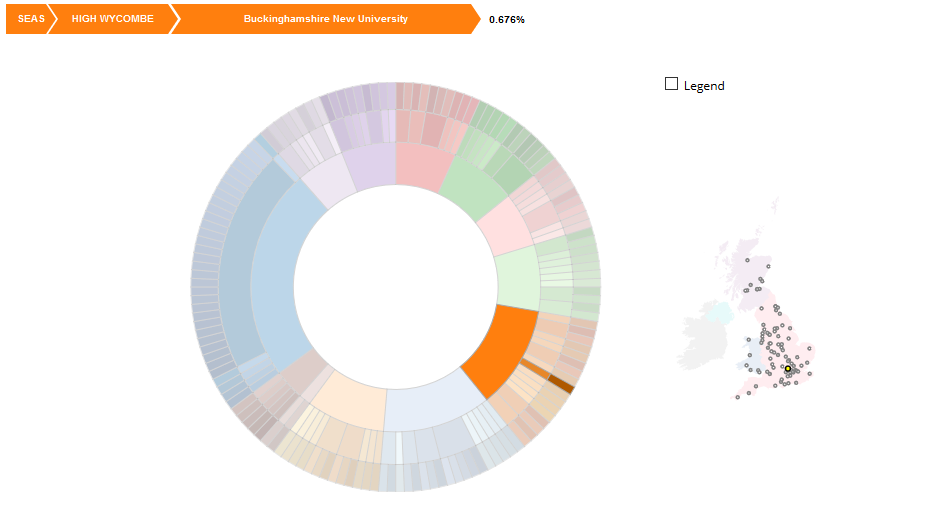
\includegraphics[width=0.3\textwidth]{imgs/Layout_SB.PNG}} 
 & This layout uses the `d3 nest' functionality with the first depth keyed to regions, the second depth keyed to towns and the third depth keyed to institutions. The `bread crumbs' and toggable legend use this data. The smaller UK map layout takes in a data set for towns \textbf{only}.
 & No data explicitly changes on the sunburst, however, selecting a town or region zooms it towards the root node and only its descendants are displayed as slices. The `bread crumb' trail has no transitions as to be responsive to mouse overs.
 \\ 
 \hline
 \raisebox{-\totalheight}{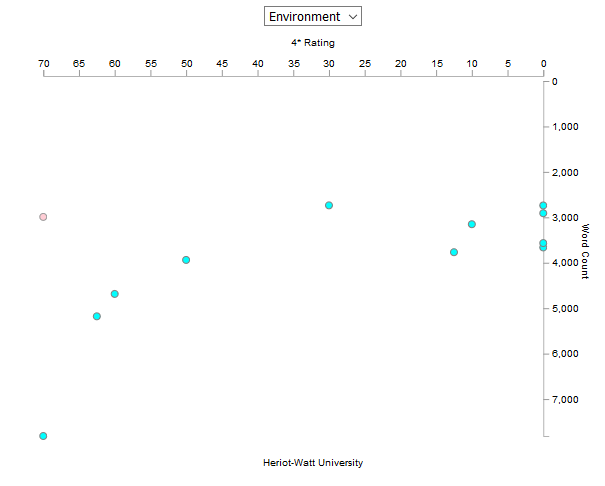
\includegraphics[width=0.3\textwidth]{imgs/Layout_SC.PNG}} 
 & This layout passes in all documents associated with a institution. This plots each point by the unique `UoAString with appended submission letters'. 
 & Topics that exist in the newly selected institution change from cyan to green and move to their new location. Removed topics turn grey with half opacity and move to the bottom right corner and disappear. New topics move in from the top left corner. 
 \\
 \hline
 \raisebox{-\totalheight}{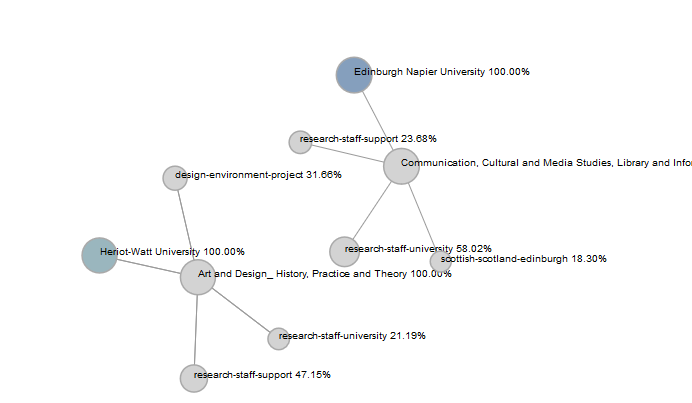
\includegraphics[width=0.3\textwidth]{imgs/Layout_NL.PNG}} 
 & This layout appends documents and refactors them into nodes with my custom addNode function. This is necessary due to how this type of graph works. It must be able to generate links between these nodes and understand their links in a flat data set. 
 & The addition of nodes move in from the top left corner and join onto existing root nodes, or make their own ones. Removal of any node fades the node and all its children out. 
 \\ [1ex] 
 \hline
\end{tabular}
\end{center}

\newpage
\subsection{Interaction between Layouts}
%This section will use images, arrows and short textual descriptions to describe the interactions between charts. Short narratives describing the rationale for these interactions should be provided.
\subsubsection{Sunburst Contained Interaction}
\begin{figure}[hbt!]
	\centering
      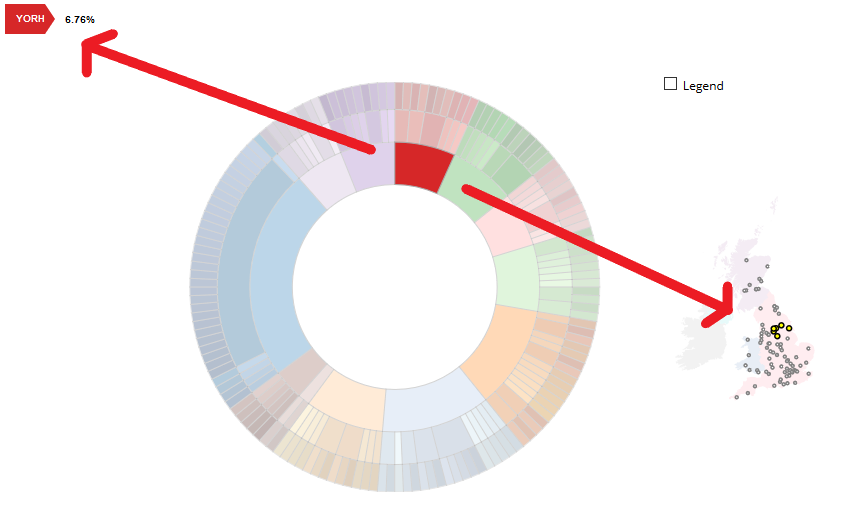
\includegraphics[width=0.6\textwidth]{imgs/sb_int/Region_select.png} \\
	\caption{Sunburst Map Highlight and Bread Crumb Trail: 
	\textit{(a)} Mouse over region highlights all towns in region on the map
	\textit{(b)} Mouse over anything displays hierarchy bread crumb trail}
	\label{fig:sb_con:reg_bread}
          \noindent\makebox[\linewidth]{\rule{\textwidth}{0.4pt}}
\end{figure}

\noindent Figure \ref{fig:sb_con:reg_bread}.a shows all towns within that region highlighted on the UK map, to represent their locations in a familiar map form. This can be used by the DoR to quickly identify where in the UK they are navigating through.

\noindent Figure \ref{fig:sb_con:reg_bread}.b shows the start of a bread crumb trail that shows the path through the descendants of the hierarchy navigation. This allows the DoR to keep track of the route he is currently navigating through.
\\

\begin{figure}[hbt!]
	\centering
      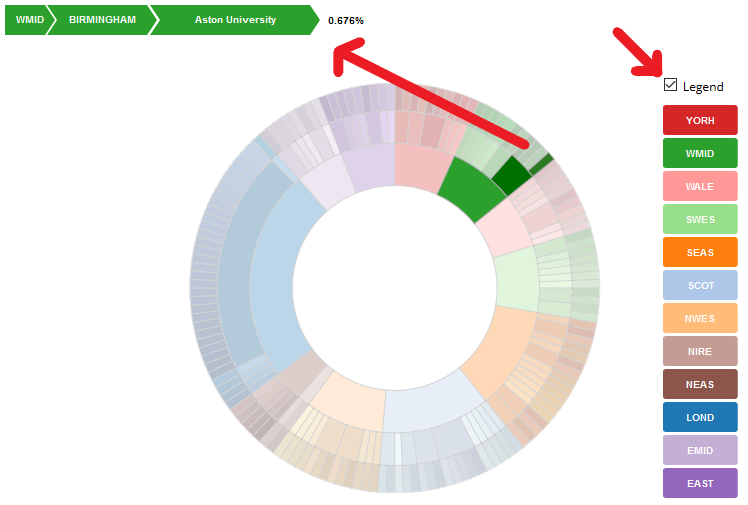
\includegraphics[width=0.5\textwidth]{imgs/sb_int/Legend_Toggle_Bread.png} \\
	\caption{Sunburst Legend Toggle: 
	\textit{(a)} Toggle checkbox to swap map with colour legend
	\textit{(b)} Mouse over anything displays hierarchy bread crumb trail}
    \label{fig:sb_con:legend_toggle_bread}
     \noindent\makebox[\linewidth]{\rule{\textwidth}{0.4pt}}
\end{figure}

\noindent Figure \ref{fig:sb_con:legend_toggle_bread}.a swaps the UK map out with a legend. This allows the DoR to also identify which region belongs to what colour. An important point is that each descendant of a region corresponds with a darker colour from the region.

\noindent Figure \ref{fig:sb_con:legend_toggle_bread}.b is similar to figure \ref{fig:sb_con:reg_bread}.b. See example above.



\begin{figure}[hbt!]
	\centering
      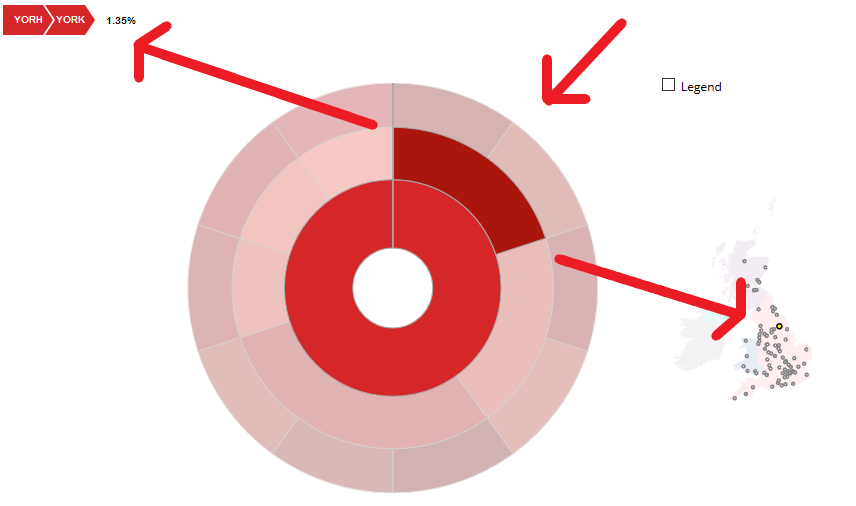
\includegraphics[width=0.6\textwidth]{imgs/sb_int/zoomable_sb.png} \\
	\caption{Sunburst Zoomable: 
	\textit{(a)} Left-click on any region or town to place it as root node}
    \label{fig:sb_con:zoomable_sb}
     \noindent\makebox[\linewidth]{\rule{\textwidth}{0.4pt}}
\end{figure}

\noindent Figure \ref{fig:sb_con:zoomable_sb}.a zooms the sunburst by selecting a region or town. This allows the DoR to filter the sunburst and focus on institutions in specific geographical areas. The UK map will only show specific towns in that region when mousing over the sunburst.

\newpage
\subsubsection{Scatter Plot Contained Interaction}
\begin{figure}[hbt!]
	\centering
      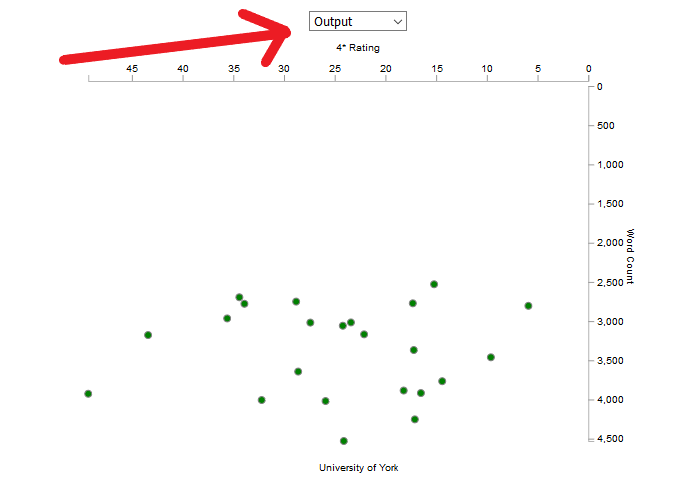
\includegraphics[width=0.6\textwidth]{imgs/sp_int/change_data.png} \\
	\caption{Scatter Plot Change Data: 
	\textit{(a)} Swap between Environment and Output}
    \label{fig:sp_con:swap_data}
     \noindent\makebox[\linewidth]{\rule{\textwidth}{0.4pt}}
\end{figure}

\noindent Figure \ref{fig:sp_con:swap_data}.a allows the swapping of 4* rating data between environment and output. This allows the DoR to compare against the specific types of rating data, giving insights of the various different types of ratings.


\subsubsection{Linked Nodes Contained Interaction}
\begin{figure}[hbt!]
	\centering
      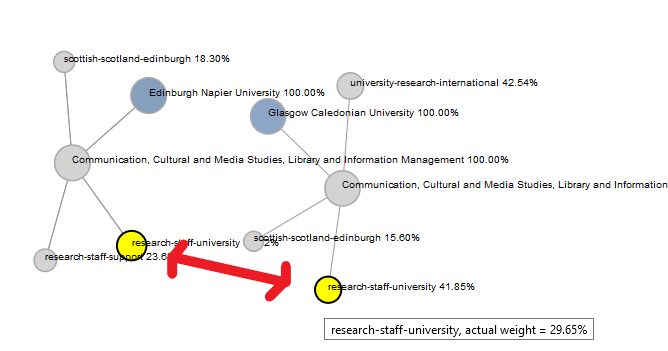
\includegraphics[width=0.6\textwidth]{imgs/ln_int/topic_weight_highlight.png} \\
	\caption{Linked Node Highlights: 
	\textit{(a)} Highlight common word combinations between topics}
    \label{fig:lp_con:common_topic_words}
     \noindent\makebox[\linewidth]{\rule{\textwidth}{0.4pt}}
\end{figure}

\noindent Figure \ref{fig:lp_con:common_topic_words}.a highlights word collections between all the topics. This is useful for the DoR as he may analyse a unit of assessment from multiple institutions, like the example above. This allows these topic words and weightings to be easily identifiable, allowing comparison of relative and actual topic weightings. This can be used with multiple institutions. \\


\begin{figure}[hbt!]
	\centering
      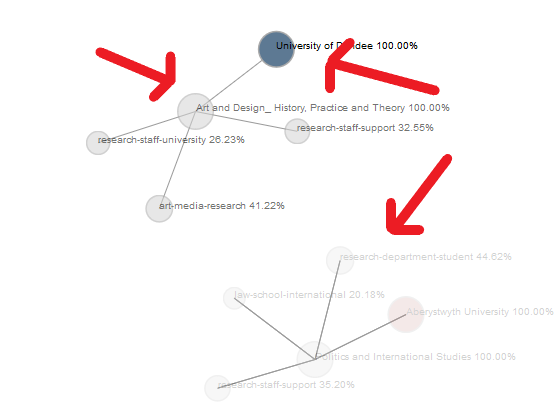
\includegraphics[width=0.6\textwidth]{imgs/ln_int/remove_nodes.png} \\
	\caption{Linked Node Fade: 
	\textit{(a)} Removal of unit and child nodes while institution remains.
	\textit{(b} Removal of all nodes.}
    \label{fig:lp_con:remove_nodes}
     \noindent\makebox[\linewidth]{\rule{\textwidth}{0.4pt}}
\end{figure}

\noindent Figure \ref{fig:lp_con:remove_nodes}.a shows the right-click interaction to remove a unit node and all children from the linked node graph, which the institution node remains. Figure \ref{fig:lp_con:remove_nodes}.b shows the removal of an institution node. This is helpful for a DoR after no longer requiring a certain word collection, topic or institution.

\subsubsection{Sunburst to Scatter Plot Interaction}

\begin{figure}[hbt!]
	\centering
      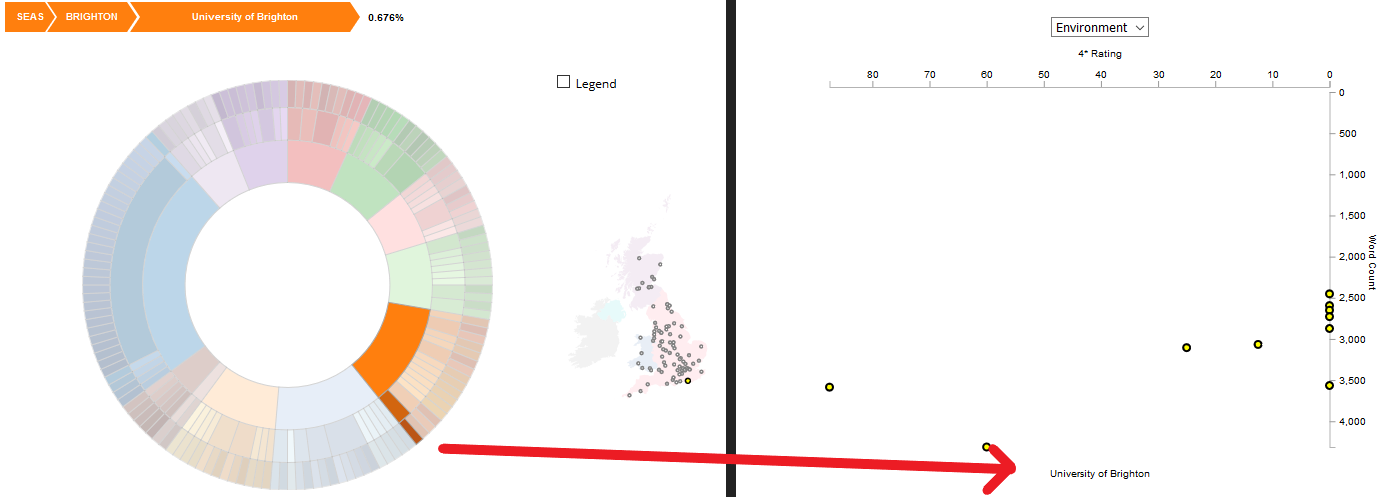
\includegraphics[width=\textwidth]{imgs/sb_sc_int/SB_SC_changedata.png} \\
	\caption{Sunburst Click Institution: 
	\textit{(a)} Change units on scatter plot by clicking on institution.}
    \label{fig:sb_sc_int:changedata}
     \noindent\makebox[\linewidth]{\rule{\textwidth}{0.4pt}}
\end{figure}

\noindent Figure \ref{fig:sb_sc_int:changedata}.a shows the left-click interaction to change to selected institution's unit data. This is helpful for a DoR to swap between institutions unit selection.


\subsubsection{Scatter Plot to Sunburst Interaction}
\begin{figure}[hbt!]
	\centering
      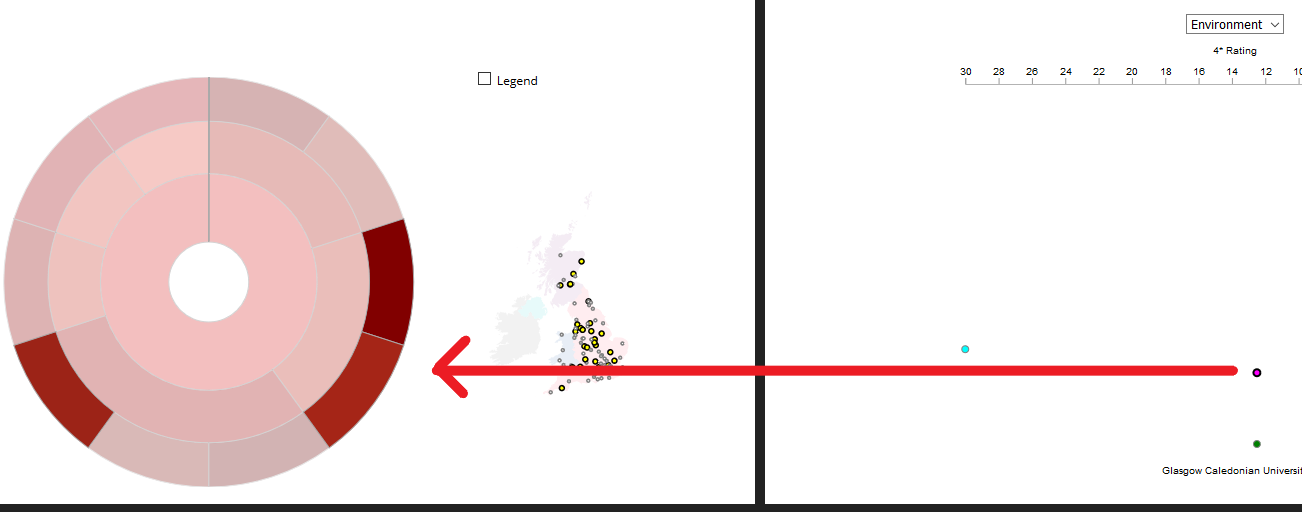
\includegraphics[width=0.6\textwidth]{imgs/sc_sb_int/select_UoA_and_compare.png} \\
	\caption{Scatter Plot Selection \& Comparison: 
	\textit{(a)} Right-click on a unit of assessment highlights it is selected.}
    \label{fig:sc_sb_int:uoa_select}
    \noindent\makebox[\linewidth]{\rule{\textwidth}{0.4pt}}
\end{figure}


\noindent Figure \ref{fig:sc_sb_int:uoa_select}.a requires a right-click to highlight a point in magenta and disables all other interactions with that point. This also freezes the sunburst to display what institutions have the selected unit of assessment. Now selecting an institution from the sunburst will only pull the selected topics data onto the scatter plot to allow for easy comparison. After performing this action the point on the scatter plot will reset so it will be removed on the next institution selection. This is useful for the DoR to allow for quick reference to what institutions have a document for the selected unit. This can provide clear comparisons of their 4* ratings.


\subsubsection{Scatter Plot to Linked Node Interaction}
\begin{figure}[hbt!]
	\centering
      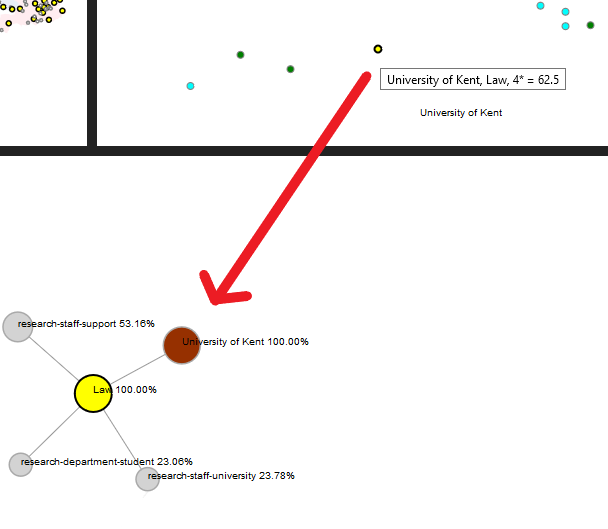
\includegraphics[width=0.4\textwidth]{imgs/sc_ln_int/SC_LN_create_node.png} \\
	\caption{Scatter Plot Create Node: 
	\textit{(a)} Clicking on scatter plot point creates node.}
    \label{fig:sc_ln_int:create_node}
     \noindent\makebox[\linewidth]{\rule{\textwidth}{0.4pt}}
\end{figure}

\noindent Figure \ref{fig:sc_ln_int:create_node}.a creates a node by clicking on a point. This is useful to the DoR by adding in more units to compare against. This can add multiple units from the same or different institution and append each to the root node.



\subsubsection{Linked Node to Sunburst Interaction}
\begin{figure}[hbt!]
	\centering
      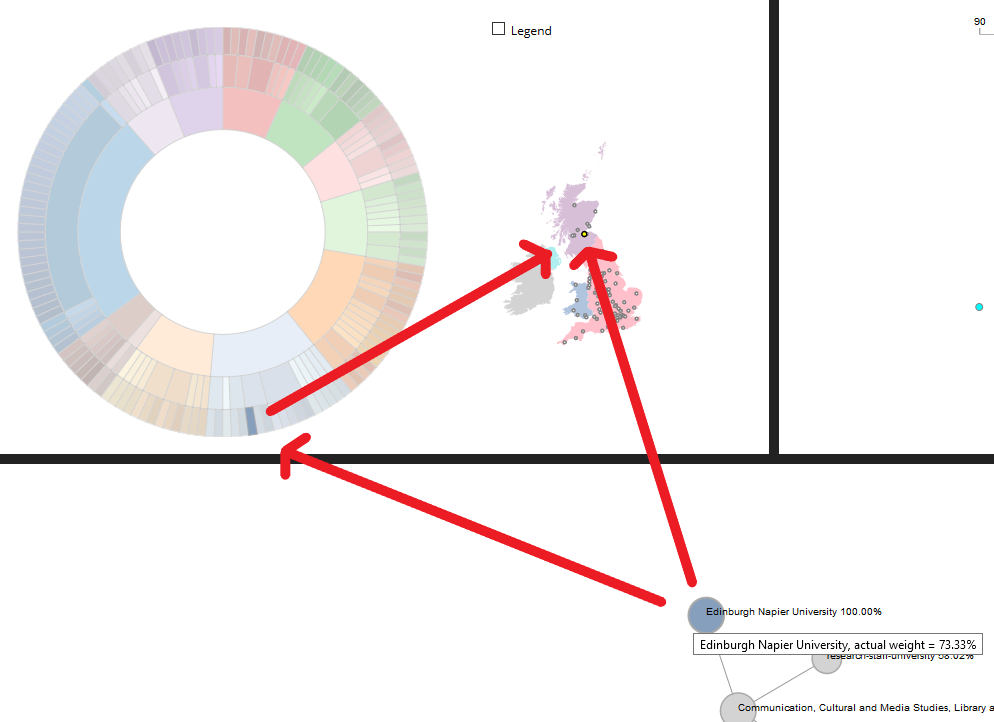
\includegraphics[width=0.6\textwidth]{imgs/sb_ln_int/LN_SB_Institute_map_highlight.png} \\
	\caption{Linked Node Highlights Institution: 
	\textit{(a)} Highlight institution on sunburst and town on the map.}
    \label{fig:ln_sb_int:institution_town_highlight}
     \noindent\makebox[\linewidth]{\rule{\textwidth}{0.4pt}}
\end{figure}

\noindent Figure \ref{fig:ln_sb_int:institution_town_highlight}.a highlights the current moused over institution on the sunburst, and highlights its location on the map. This is useful for the DoR to easily identify where on the sunburst the institution is positioned, while also feeding back its geographical location.


\subsubsection{Sunburst, Scatter Plot and Linked Node Interactions}
\begin{figure}[hbt!]
	\centering
      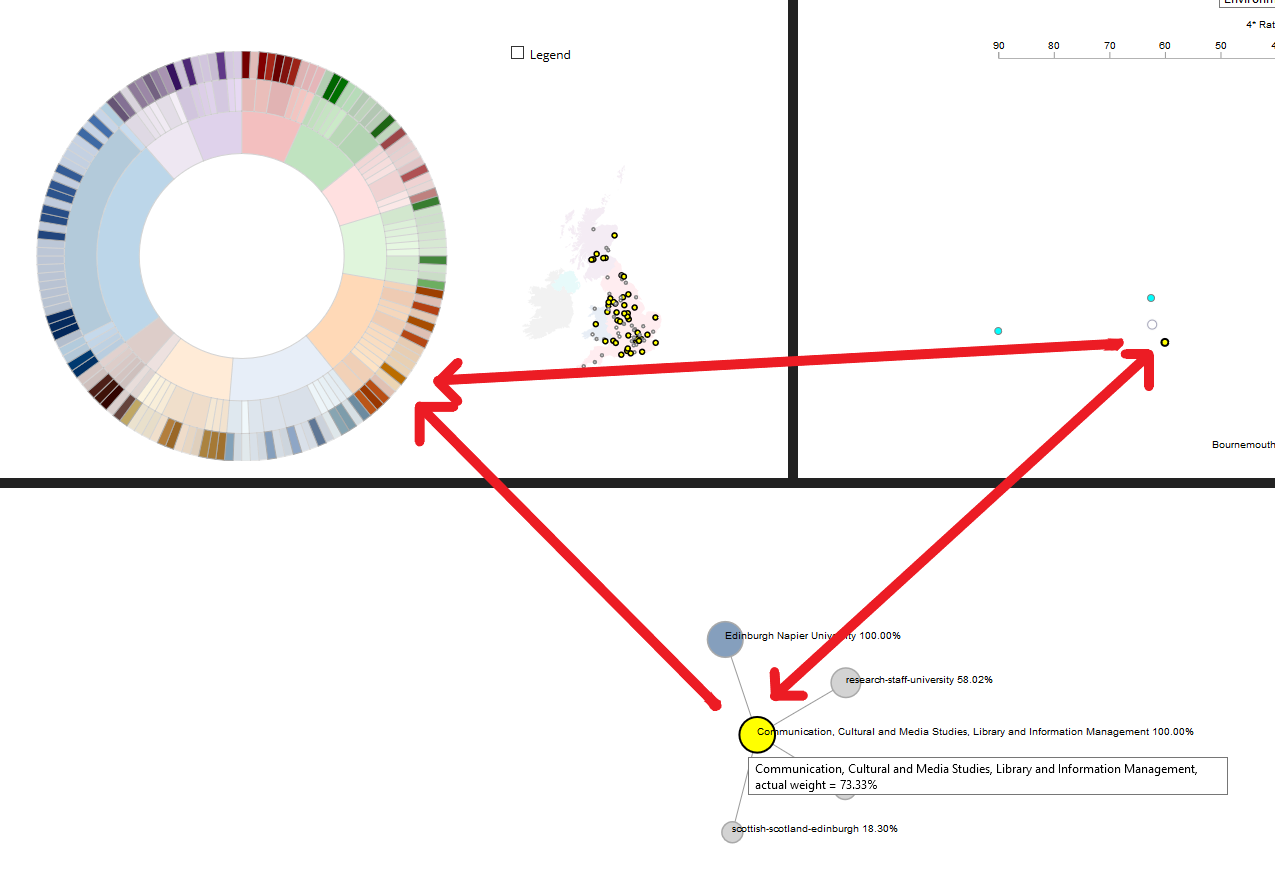
\includegraphics[width=0.55\textwidth]{imgs/sb_sc_ln_int/3_way_topic_highlight.png} \\
	\caption{Unit of Assessment Highlights: 
	\textit{(a)} Mouse over on Linked Node unit highlights same unit on scatter plot and every institution that contains that unit on the sunburst.
	\textit{(b)} Same as \ref{fig:sb_sc_ln_int:3_way_topic_highlight}.a but mouse over on scatter plot point highlights same unit on linked node.}
    \label{fig:sb_sc_ln_int:3_way_topic_highlight}
     \noindent\makebox[\linewidth]{\rule{\textwidth}{0.4pt}}
\end{figure}

\noindent Figure \ref{fig:sb_sc_ln_int:3_way_topic_highlight}.a and \ref{fig:sb_sc_ln_int:3_way_topic_highlight}.b highlights where this unit of assessment is present on the scatter plot or the linked node respectively. Mousing over a unit on either graph displays what institution this unit is present in on the sunburst. This is useful for the DoR as it shows quickly what institution has a document based on that unit. It also allows to quick display where each document is on the scatter plot and linked node graph. This can especially be useful, for example, to quickly locate where the the current unit moused over on the linked node graph is on the scatter plot graph. Similarly, this can check if the unit moused over on the scatter plot is currently present in the linked node graph. \\

\begin{figure}[hbt!]
	\centering
      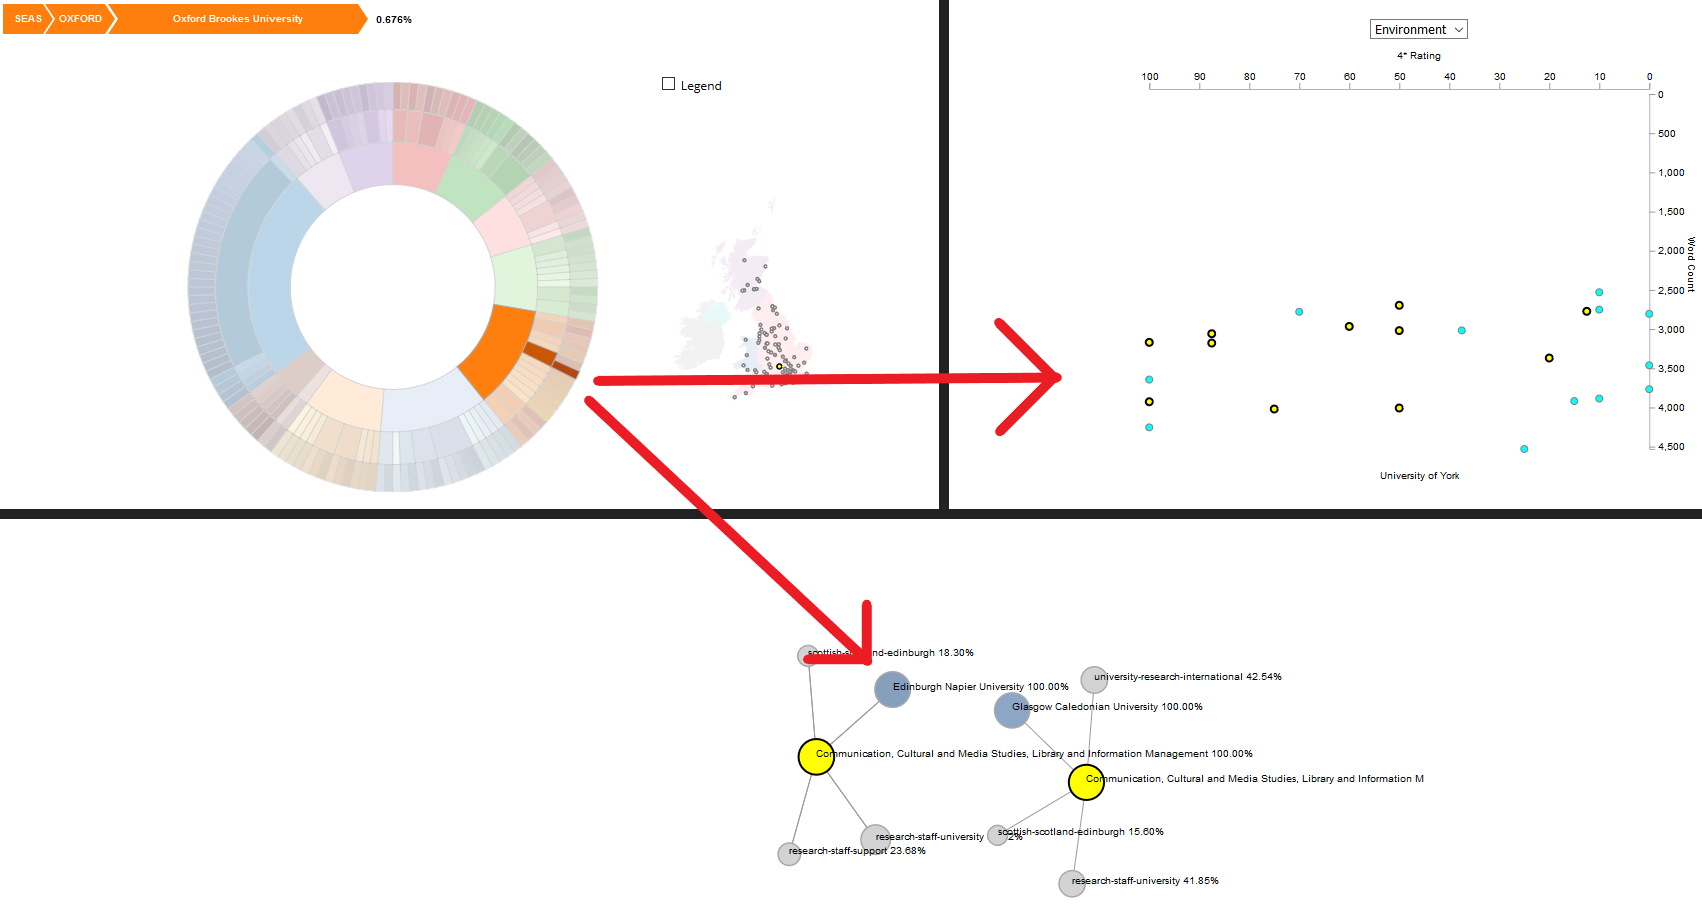
\includegraphics[width=\textwidth]{imgs/sb_sc_ln_int/topics_in_current_and_in_highlighted.png} \\
	\caption{All Unit of Assessment Highlights: 
	\textit{(a)} Mouse over on sunburst institution highlights all the units which are also currently present on the scatter plot and linked node graph.}
    \label{fig:sb_sc_ln_int:topics_in_cur_mouse}
     \noindent\makebox[\linewidth]{\rule{\textwidth}{0.4pt}}
\end{figure}

\noindent Figure \ref{fig:sb_sc_ln_int:topics_in_cur_mouse}.a shows that when mousing over an institution on the sunburst, the units that highlight on the scatter plot and linked node graphs are also present in that institution. This is particularly helpful for the DoR as to confirm that the unit they are looking for is in the moused over institution.



\newpage
\section{Software Design}
\subsection{Design overview}
% (one page max) This should provide a diagram and short associated narrative describing the top-level structure of your design (i.e. how you have split the design up into the various source files and what their runtime equivalents communicate with each other).

\begin{center}
 \begin{tabular}{||c|p{0.65\linewidth}||} 
 \hline
 Project Stucture & Description \\ [0.5ex] 
 \hline\hline
 \raisebox{-\totalheight}{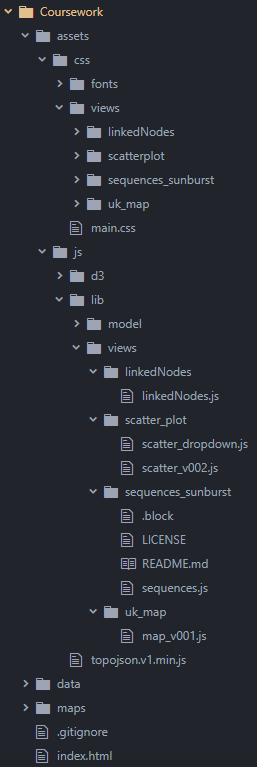
\includegraphics[width=0.3\textwidth]{imgs/project_struct/project_structure.png}} 
 & 
 This project is based off a modular design. All charts are within the \textbf{`./js/lib/views/'} and matching to their own folder. These files are imported into the \textbf{`./index.html'} file. This file corresponds with the initialisation function presented by Chantler. This file also contains global functions that each modular code imported can utilise. These functions work with variables assigned to the modular charts and are used to render data and display interactions.
 
 Each chart also has its own corresponding css file in \textbf{`./css/views/'} with their own folder. This allows to easily change specific highlighting designs, and is also imported into the \textbf{`./index.html'} file.
 \\ 
 \hline
\end{tabular}
\end{center}


\newpage
\subsection{Use of Design Patterns}
% This section should briefly describe any software design patterns that you have used. Each design pattern (together with a critical analysis of what their advantages and disadvantages were for your project) should be described in their own, short, numbered subsection (4.2.1, 4.2.2 … etc.)
\subsubsection{Function Class}
A prevalent software design pattern for this project was a function class. This is essentially a function imitating a class definition. This has its advantages such as providing information hiding techniques and assigning variables locally for that class. This means variables cannot accidentally be modified else where in this project. Another benefit of this allows for overrides of specific functions of variables when explicitly stated. For example, updating an accessor function when changing data on my scatter plot chart (See figure \ref{fig:sc_sb_int:uoa_select}). This also allowed for function chaining by continually returning an object from each public method.

This has disadvantages however, by not allowing to return data explicitly when chaining multiple functions. This required the use of d3's select function to get data from DOM elements instead, which is not as efficient as direct access to a basic `getter' function.

\subsubsection{Global Functions}
Assigning global helper functions in the main \textbf{`./index.html'} allowed for cleaner syntax and less code repetition between charts. An example of this is `resetting' charts after modifying specific elements. This function quickly returned interacted elements back to their default state with one function call. This reduced development time greatly without constant implementation of these functions for individual charts.

\subsubsection{Function Callbacks}
This project has numerous amounts of function callbacks to handle functionality cleanly. This is also beneficial for changing what these functions do on the fly. This was useful in my project when I swap my x-axis data plots from `environment' to `output'. It was also beneficial for disabling mouse click and mouse over functionality when selecting a topic from my scatter plot.




\section{Original contribution made by the student}
\subsection{Highlights} 
% This section should briefly identify and highlight anything that you feel particularly proud of that you would like to bring to the attention of the examiners. 
\subsubsection{Linked Node Implementation}
I am particularly proud of this chart design as I implemented a node creation function that fitted document data into the flat data set required by this layout (See \textbf{`addNodes()'} in \textbf{`linkedNode.js'}). I also implemented traversal functions to update node weights on addition or deletion, delete specific nodes and delete all their children nodes (See \textbf{`removeNodeAndChildren()'} and \textbf{`updateWeights()'} in \textbf{`linkedNode.js'}).

\subsubsection{Scatter Plot Selection Implementation}
I implemented a point selection function on the scatter plot graph to allow comparison of two or more units when selecting another institution. This kept the current point in the graph and filtered the new incoming data to only allow the selected unit (See \textbf{`checkAnySelected()'} and \textbf{`rightClickFunction()'} in \textbf{`sequences.js'}).

\subsubsection{Bread Crumb Trail Scale to Words}
I modified the bread crumb implementation to allow the sizing to fit the displayed word when it is rendered with. This did not come with the original implementation of this sunburst (See \textbf{`updateBreadcrumbs()'} in \textbf{`sequences.js'}).

\subsection{File by File description}
% A subsection should be provided for each of your application’s software source files (e.g. 5.2.1, 5.2.2, etc,). The subsections should have the same name as the source files. They should start with a table indicating the percentage contributions of the sources, and if applicable, the source of the code and its licence as shown in the example below:


\subsubsection{index.html}
\begin{center}
 \begin{tabular}{||p{0.15\textwidth}|p{0.15\textwidth}|p{0.15\textwidth}|p{0.15\textwidth}|p{0.15\textwidth}||} 
 \hline
 Contribution by student & Contribution from course & contribution from 3rd party & Source & Licence 
 \\
 \hline
 40\% & 60\% & 0\% &  &
 \\
 \hline
\end{tabular}
\end{center}
I implemented many extra interaction functions for selection towards the bottom of the file to ease development.

\subsubsection{sequences.js}
\begin{center}
 \begin{tabular}{||p{0.15\textwidth}|p{0.15\textwidth}|p{0.15\textwidth}|p{0.15\textwidth}|p{0.15\textwidth}||} 
 \hline
 Contribution by student & Contribution from course & contribution from 3rd party & Source & Licence 
 \\
 \hline
 43\% & 10\% & 47\% & Block 766f8f6d31f645 c39f488a0befa 1e3c8, Block 1a3f8e44cdcb3 054121dfd991f 59fbc2 & Apache 2.0, GNU General Public License, version 3
 \\
 \hline
\end{tabular}
\end{center}
I heavily modified the original file to correspond with the same setup used in the course. This allows me to understand how this view works as well as showing understanding of methods learned during this course. I also implemented the zooming function provided by the second source. I originally gave my contribution as 40\%, the course as 10\% and sources as 50\%, but I also implemented a toggle feature for the map in this file so that is why the contribution is higher than my original 40\% rating.


\subsubsection{scatter\_v002.js}
\begin{center}
 \begin{tabular}{||p{0.15\textwidth}|p{0.15\textwidth}|p{0.15\textwidth}|p{0.15\textwidth}|p{0.15\textwidth}||} 
 \hline
 Contribution by student & Contribution from course & contribution from 3rd party & Source & Licence 
 \\
 \hline
 35\% & 65\% & 0\% & & 
 \\
 \hline
\end{tabular}
\end{center}
I implemented extra functionality, such as point selection for units. I also added in extra labels for the axises and bottom of the grid. I swapped the axis orientations from left and bottom to right and top. I also added the drop down bar from another lab, however it is part of the course.

\subsubsection{scatter\_dropdown.js}
\begin{center}
 \begin{tabular}{||p{0.15\textwidth}|p{0.15\textwidth}|p{0.15\textwidth}|p{0.15\textwidth}|p{0.15\textwidth}||} 
 \hline
 Contribution by student & Contribution from course & contribution from 3rd party & Source & Licence 
 \\
 \hline
 0\% & 100\% & 0\% & & 
 \\
 \hline
\end{tabular}
\end{center}


\subsubsection{linkedNodes.js}
\begin{center}
 \begin{tabular}{||p{0.15\textwidth}|p{0.15\textwidth}|p{0.15\textwidth}|p{0.15\textwidth}|p{0.15\textwidth}||} 
 \hline
 Contribution by student & Contribution from course & contribution from 3rd party & Source & Licence 
 \\
 \hline
 65\% & 10\% & 25\% & Block 1129492, Block 6c282b65246f8 f46bb55aadc32 2db709 &  GNU General Public License, version 3
 \\
 \hline
\end{tabular}
\end{center}
I heavily modified the original file to correspond with the same setup used in the course. This allows me to understand how this view works as well as showing understanding of methods learned during this course. I also modified the code to implement node creation when new documents were added in. I also added methods to manipulate nodes, such as modify the weight, scaling them correctly, deletion of nodes and there children and addition of labels onto nodes.


\subsubsection{map\_v001.js}
\begin{center}
 \begin{tabular}{||p{0.15\textwidth}|p{0.15\textwidth}|p{0.15\textwidth}|p{0.15\textwidth}|p{0.15\textwidth}||} 
 \hline
 Contribution by student & Contribution from course & contribution from 3rd party & Source & Licence 
 \\
 \hline
 2\% & 98\% & 0\% &  & 
 \\
 \hline
\end{tabular}
\end{center}
I only modified the scaling of the map for this file.



%This should be followed by a short description of the student’s contribution to the module (source file). If the student’s contribution to a particular source file is 0\% then,  no narrative is required.

\newpage
\section*{Source code listings}
\subsection{index.html}
\inputminted{html}{source/index.html}

\newpage
\subsection{sequences.js}
\inputminted{js}{source/sequences.js}

\newpage
\subsection{map\_v001.js}
\inputminted{js}{source/map_v001.js}

\newpage
\subsection{scatter\_v002.js}
\inputminted{js}{source/scatter_v002.js}

\newpage
\subsection{scatter\_dropdown.js}
\inputminted{js}{source/scatter_dropdown.js}

\newpage
\subsection{linkedNodes.js}
\inputminted{js}{source/linkedNodes.js}


\newpage
\subsection{main.css}
\inputminted{css}{source/main.css}


\newpage
\subsection{sequences.css}
\inputminted{css}{source/sequences.css}


\newpage
\subsection{map\-v001.css}
\inputminted{css}{source/map-v001.css}


\newpage
\subsection{scatterplot.css}
\inputminted{css}{source/scatterplot.css}

\newpage
\subsection{linkedNodes.css}
\inputminted{css}{source/linkedNodes.css}

\end{document}
